% !TEX root =  ../supplementary.tex
\section{A Bivariate Joint Model for the Longitudinal PSA, and DRE Measurements, and Time to Cancer Progression}
\label{sec:jm_framework}

In this appendix section, we first provide an introduction to the world's largest active surveillance (AS) program called Prostate Cancer Research International Active Surveillance, abbreviated as PRIAS \citep{bokhorst2016decade}, that we use to develop our methodology. We then present an introduction to the joint models for time-to-event and longitudinal data \citep{tsiatis2004joint,rizopoulos2012joint}, that we fit to the PRIAS dataset. Lastly, we present the parameter estimation for our model using the Bayesian approach. 

\subsection{PRIAS Dataset}
To develop our methodology we use the data of prostate cancer patients from the world's largest AS study called PRIAS \cite{bokhorst2016decade}. More than 100 medical centers from 17 countries worldwide contribute to the collection of data, utilizing a common study protocol and a web-based tool, both available at \url{www.prias-project.org}. We use data collected over a period of ten years, between December 2006 (beginning of PRIAS study) and December 2016. It consists of 5270 patients. The primary event of interest in this work is cancer progression detected upon a positive biopsy. It is observed in 866 patients, although the time of cancer progression is interval censored because biopsies are scheduled periodically. Biopsies are scheduled at the  following fixed follow-up times (measured since inclusion in AS): year 1, 4, 7, and 10, and every 5 years thereafter. An annual schedule of biopsies is prescribed to those patients who have a PSA doubling time between 0 and 10 years. The PSA doubling time at any point during follow-up is measured as the inverse of the slope of the regression line through the base two logarithm of the observed PSA values. There are three types of competing events, namely death of 63 patients, of which 61 died from non prostate cancer related reasons; removal of 464 patients from AS on the basis of their observed DRE and PSA measurements; and loss to follow-up of 685 patients because of patient anxiety or unknown reasons. In this work, we assume these three types of events to be censoring (see \ref{subsec:ascertainment_bias} for details). However, our model allows removal of patients to depend on observed longitudinal data and baseline covariates of the patient. Under the aforementioned assumption of censoring, Figure~\ref{fig:npmle_plot} shows the cumulative risk of cancer progression over the study follow-up period. Prostate cancer is a slowly progressing disease, which is evident by the large proportion of patients not having a cancer progression by the end of the ten year follow-up period.

\begin{figure}[!htb]
\captionsetup{justification=justified}
\centerline{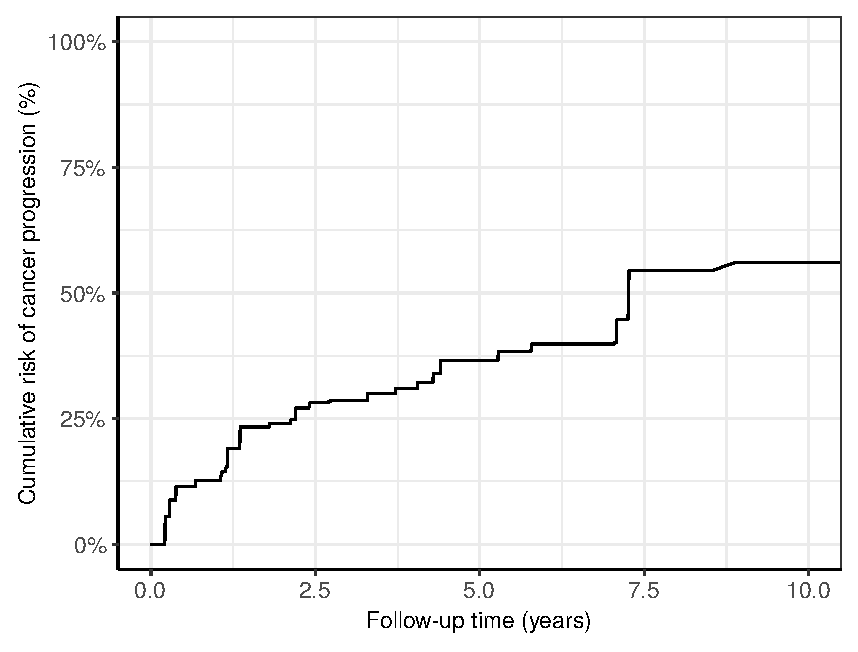
\includegraphics[width=\columnwidth]{images/npmle_plot.eps}}
\caption{\textbf{Estimated cumulative risk of cancer progression in AS} for patients in the Prostate Cancer Research International Active Surveillance (PRIAS) dataset. Nearly 50\% patients (\textit{slow progressing}) do not progress in the ten year follow-up period. Cumulative risk is estimated using nonparametric maximum likelihood estimation \citep{turnbull1976empirical}, to account for interval censored cancer progression times observed in PRIAS program. Censoring includes death, removal from AS on the basis of observed longitudinal data, and patient dropout.}
\label{fig:npmle_plot}
\end{figure}

For all patients, PSA measurements (ng/mL) are scheduled every 3 months for the first 2 years and every 6 months thereafter. The DRE measurements (ordinal scale) are scheduled every 6 months. We use the DRE measurements after converting them to a binary scale, namely $\mbox{DRE} > \mbox{T1c}$ and $\mbox{DRE} = \mbox{T1c}$. A DRE measurement equal to T1c \citep{schroder1992tnm} indicates a clinically inapparent tumor which is not palpable or visible by imaging. Tumors with $\mbox{DRE} > \mbox{T1c}$ are palpable. On average 5 DRE and 9 PSA measurements have been recorded per patient. 

\subsection{Model Definition}
\label{subsec:model_def}
Let $T_i^*$ denote the true cancer progression time of the ${i\mbox{-th}}$ patient included in PRIAS. Since biopsies are conducted periodically, $T_i^*$ is observed with interval censoring ${l_i < T_i^* \leq r_i}$. When progression is observed for the patient at his latest biopsy time $r_i$, then $l_i$ denotes the time of the second latest biopsy. Otherwise, $l_i$ denotes the time of the latest biopsy and ${r_i=\infty}$. Let $\boldsymbol{y}_{di}$ and $\boldsymbol{y}_{pi}$ denote his observed DRE and PSA longitudinal measurements, respectively. The observed data of all $n$ patients is denoted by ${\mathcal{D}_n = \{l_i, r_i, \boldsymbol{y}_{di}, \boldsymbol{y}_{pi}; i = 1, \ldots, n\}}$.

\begin{figure}[!htb]
\captionsetup{justification=justified}
\centerline{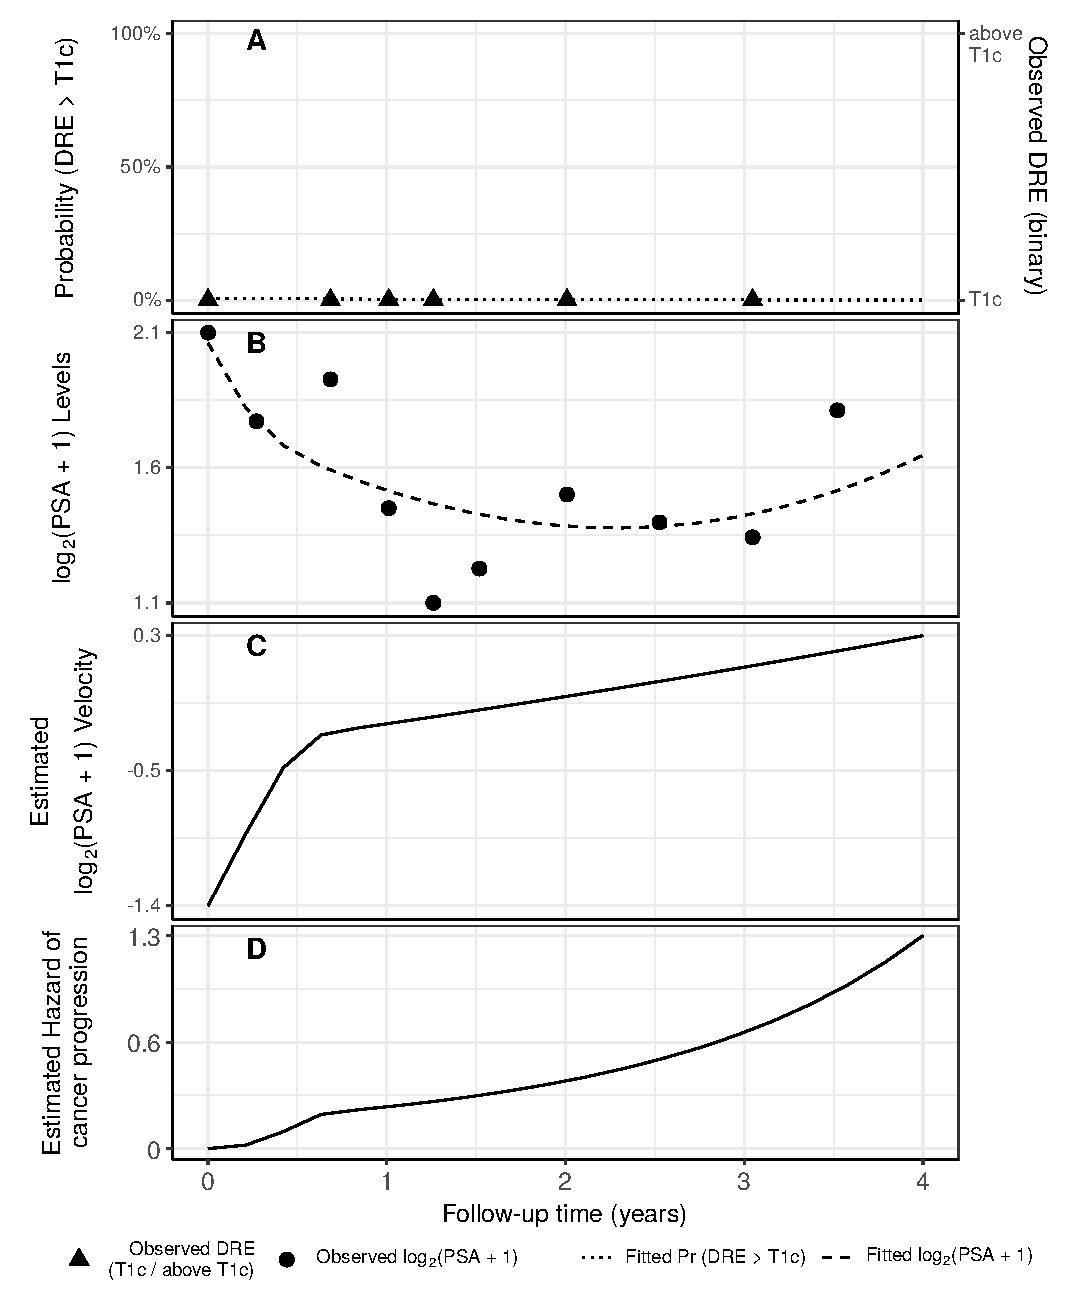
\includegraphics[width=\columnwidth]{images/jmExplanationPlot_1757.eps}}
\caption{\textbf{Illustration of the joint model fitted to the PRIAS dataset}. \textbf{Panel~A:} shows the observed DRE measurements and the fitted probability of obtaining $\mbox{DRE} > \mbox{T1c}$ (Equation~\ref{eq:long_model_dre}) for . \textbf{Panel~B:} shows the observed and fitted $\log_2(\mbox{PSA} + 1)$ measurements (Equation~\ref{eq:long_model_psa}). \textbf{Panel~C:} shows the estimated $\log_2(\mbox{PSA} + 1)$ velocity (velocity cannot be observed directly) over time. The hazard function (Equation~\ref{eq:rel_risk_model}) shown in \textbf{Panel~D}, depends on the fitted log odds of having a $\mbox{DRE} > \mbox{T1c}$, and the fitted $\log_2(\mbox{PSA} + 1)$ value and velocity.}
\label{fig:jmExplanationPlot_1757}
\end{figure}

In our joint model, the patient-specific DRE and PSA measurements over time are modeled using a bivariate generalized linear mixed effects sub-model. The sub-model for DRE is given by (see Panel~A, Figure~\ref{fig:jmExplanationPlot_1757}):
\begin{equation}
\label{eq:long_model_dre}
\begin{split}
    \mbox{logit} \big[\mbox{Pr}\{y_{di}(t) > \mbox{T1c}\}\big] &= \beta_{0d} + b_{0di} + (\beta_{1d} + b_{1di}) t\\
    &+ \beta_{2d} (\mbox{Age}_i-70) + \beta_{3d} (\mbox{Age}_i-70)^2
    \end{split}
\end{equation}
where, $t$ denotes the follow-up visit time, and $\mbox{Age}_i$ is the age of the ${i\mbox{-th}}$ patient at the time of inclusion in AS. The fixed effect parameters are denoted by ${\{\beta_{0d}, \ldots, \beta_{3d}\}}$, and ${\{b_{0di}, b_{1di}\}}$ are the patient specific random effects. With this definition, we assume that the patient-specific log odds of obtaining a DRE measurement larger than T1c remain linear over time. 

The mixed effects sub-model for PSA is given by (see Panel~B, Figure~\ref{fig:jmExplanationPlot_1757}):
\begin{equation}
\label{eq:long_model_psa}
\begin{split}
    \log_2 \big\{y_{pi}(t) + 1\big\} &= m_{pi}(t) + \varepsilon_{pi}(t),\\
    m_{pi}(t) &= \beta_{0p} + b_{0pi} + \sum_{k=1}^4 (\beta_{kp} + b_{kpi})  B_k(t,\mathcal{K})\\ 
    &+ \beta_{5p} (\mbox{Age}_i-70) + \beta_{6p} (\mbox{Age}_i-70)^2,
    \end{split}
\end{equation}
where, $m_{pi}(t)$ denotes the underlying measurement error free value of $\log_2 (\mbox{PSA} + 1)$ transformed \citep{pearson1994mixed,lin2000latent} measurements at time $t$. We model it non-linearly over time using B-splines \citep{de1978practical}. To this end, our B-spline basis function $B_k(t, \mathcal{K})$ has 3 internal knots at $\mathcal{K} = \{0.1, 0.7, 4\}$ years, and boundary knots at 0 and 5.42 years (95-th percentile of the observed follow-up times). The fixed effect parameters are denoted by ${\{\beta_{0p},\ldots,\beta_{6p}\}}$, and ${\{b_{0pi}, \ldots, b_{4pi}\}}$ are the patient specific random effects. The error $\varepsilon_{pi}(t)$ is assumed to be t-distributed with three degrees of freedom (see Appendix~B.1) and scale $\sigma$, and is independent of the random effects. 

To account for the correlation between the DRE and PSA measurements of a patient, we link their corresponding random effects. More specifically, the complete vector of random effects ${\boldsymbol{b}_i = (b_{0di}, b_{1di}, b_{0pi}, \ldots, b_{4pi})^T}$ is assumed to follow a multivariate normal distribution with mean zero and variance-covariance matrix $\boldsymbol{D}$.

To model the impact of DRE and PSA measurements on the risk of cancer progression, our joint model uses a relative risk sub-model. More specifically, the hazard of cancer progression $h_i(t)$ at a time $t$ is given by (see Panel~D, Figure~\ref{fig:jmExplanationPlot_1757}):
\begin{equation}
\label{eq:rel_risk_model}
\begin{split}
    h_i(t) &= h_0(t) \exp\Big(\gamma_1 (\mbox{Age}_i-70) + \gamma_2 (\mbox{Age}_i-70)^2\\
    &+\alpha_{1d} \mbox{logit} \big[\mbox{Pr}\{y_{di}(t) > \mbox{T1c}\}\big]+ \alpha_{1p} m_{pi}(t) + \alpha_{2p} \frac{\partial m_{pi}(t)}{\partial {t}}\Big),
    \end{split}
\end{equation}
where, $\gamma_1, \gamma_2$ are the parameters for the effect of age. The parameter $\alpha_{1d}$ models the impact of log odds of obtaining a $\mbox{DRE} > \mbox{T1c}$ on the hazard of cancer progression. The impact of PSA on the hazard of cancer progression is modeled in two ways: a) the impact of the error free underlying PSA value $m_{pi}(t)$ (see Panel~B, Figure~\ref{fig:jmExplanationPlot_1757}), and b) the impact of the underlying PSA velocity $\partial m_{pi}(t)/\partial {t}$ (see Panel~C, Figure~\ref{fig:jmExplanationPlot_1757}). The corresponding parameters are $\alpha_{1p}$ and $\alpha_{2p}$, respectively. Lastly, $h_0(t)$ is the baseline hazard at time t, and is modeled flexibly using P-splines \citep{eilers1996flexible}. More specifically:
\begin{equation*}
\log{h_0(t)} = \gamma_{h_0,0} + \sum_{q=1}^Q \gamma_{h_0,q} B_q(t, \boldsymbol{v}),
\end{equation*}
where $B_q(t, \boldsymbol{v})$ denotes the $q$-th basis function of a B-spline with knots $\boldsymbol{v} = v_1, \ldots, v_Q$ and vector of spline coefficients $\gamma_{h_0}$. To avoid choosing the number and position of knots in the spline, a relatively high number of knots (e.g., 15 to 20) are chosen and the corresponding B-spline regression coefficients $\gamma_{h_0}$ are penalized using a differences penalty \citep{eilers1996flexible}. An example fitted hazard is shown in panel D of Figure~\ref{fig:jmExplanationPlot_1757}.  

\subsection{Parameter Estimation}
We estimate the parameters of the joint model using Markov chain Monte Carlo (MCMC) methods under the Bayesian framework. Let $\boldsymbol{\theta}$ denote the vector of all of the parameters of the joint model. The joint model postulates that given the random effects, the time to cancer progression, and the DRE and PSA measurements taken over time are all mutually independent. Under this assumption the posterior distribution of the parameters is given by:
\begin{align*}
p(\boldsymbol{\theta}, \boldsymbol{b} \mid \mathcal{D}_n) & \propto \prod_{i=1}^n p(l_i, r_i, \boldsymbol{y}_{di}, \boldsymbol{y}_{pi}, \mid \boldsymbol{b}_i, \boldsymbol{\theta}) p(\boldsymbol{b}_i \mid \boldsymbol{\theta}) p(\boldsymbol{\theta})\\
& \propto \prod_{i=1}^n p(l_i, r_i \mid \boldsymbol{b}_i, \boldsymbol{\theta}) p(\boldsymbol{y}_{di} \mid \boldsymbol{b}_i, \boldsymbol{\theta}) p(\boldsymbol{y}_{pi} \mid \boldsymbol{b}_i, \boldsymbol{\theta}) p(\boldsymbol{b}_i \mid \boldsymbol{\theta}) p(\boldsymbol{\theta}),\\
p(\boldsymbol{b}_i \mid \boldsymbol{\theta}) &= \frac{1}{\sqrt{(2 \pi)^q \text{det}(\boldsymbol{D})}} \exp(\boldsymbol{b}_i^T \boldsymbol{D}^{-1} \boldsymbol{b}_i),
\end{align*}
where, the likelihood contribution of the DRE outcome, conditional on the random effects is:
\begin{equation*}
p(\boldsymbol{y}_{di} \mid \boldsymbol{b}_i, \boldsymbol{\theta}) = \prod_{k=1}^{n_{di}} \frac{\exp\Big[-\mbox{logit} \big\{\mbox{Pr}(y_{dik} > \mbox{T1c})\big\} I(y_{dik}=\mbox{T1c}) \Big]}  {1+\exp\Big[-\mbox{logit} \big\{\mbox{Pr}(y_{dik} > \mbox{T1c})\big\}\Big]},
\end{equation*}
where $I(\cdot)$ is an indicator function which takes the value 1 if the $k$-th repeated DRE measurement ${y_{dik}=\mbox{T1c}}$, and takes the value 0 otherwise. The likelihood contribution of the PSA outcome, conditional on the random effects is:
\begin{equation*}
p(\boldsymbol{y}_{pi} \mid \boldsymbol{b}_i, \boldsymbol{\theta}) = \frac{1}{\big(\sqrt{2 \pi \sigma^2}\big)^{n_{pi}}} \exp\bigg(-\frac{{\lVert{\boldsymbol{y}_{pi} - \boldsymbol{m}_{pi}}\rVert}^2}{\sigma^2}\bigg),
\end{equation*}
The likelihood contribution of the time to cancer progression outcome is given by:
\begin{equation}
\label{web_eq : likelihood_contribution_survival}
p(l_i,r_i\mid \boldsymbol{b}_i,\boldsymbol{\theta}) = \exp\Big\{-\int_0^{l_i} h_i(s)\mathrm{d}{s}\Big\} - \exp\Big\{-\int_0^{r_i}h_i(s)\mathrm{d}{s}\Big\}.
\end{equation}
The integral in (\ref{web_eq : likelihood_contribution_survival}) does not have a closed-form solution, and therefore we use a 15-point Gauss-Kronrod quadrature rule to approximate it.

We use independent normal priors with zero mean and variance 100 for the fixed effects ${\{\beta_{0d},\ldots,\beta_{3d}, \beta_{0p},\ldots,\beta_{6p}\}}$, and inverse Gamma prior with shape and rate both equal to 0.01 for the parameter $\sigma^2$. For the variance-covariance matrix $\boldsymbol{D}$ of the random effects we take inverse Wishart prior with an identity scale matrix and degrees of freedom equal to 7 (number of random effects). For the relative risk model's parameters $\{\gamma_1, \gamma_2\}$ and the association parameters $\{\alpha_{1d}, \alpha_{1p}, \alpha_{2p}\}$, we use independent normal priors with zero mean and variance 100.

\subsection{Personalized Posterior Predictive Distribution of Time of Cancer Progression}
Let us assume a new patient $j$, for whom we need to make a personalized biopsy decision. Let his current follow-up visit time be $s$, latest time of biopsy be $t\leq s$, observed vectors of DRE and PSA measurements be $\mathcal{Y}_{dj}(s)$ and $\mathcal{Y}_{pj}(s)$, respectively. The combined information from the observed data is given by the following posterior predictive distribution $g(T^*_j)$ of his time of cancer progression $T^*_j$:
\begin{equation*}
\label{eq:post_pred_dist}
\begin{aligned}
g(T^*_j) &= p\big\{T^*_j \mid T^*_j > t, \mathcal{Y}_{dj}(s), \mathcal{Y}_{pj}(s), \mathcal{D}_n\big\}\\
&= \int \int p\big(T^*_j \mid T^*_j > t, \boldsymbol{b}_j, \boldsymbol{\theta}\big)\\
&\times p\big\{\boldsymbol{b}_j \mid T^*_j>t, \mathcal{Y}_{dj}(s), \mathcal{Y}_{pj}(s), \boldsymbol{\theta}\big\}p\big(\boldsymbol{\theta} \mid \mathcal{D}_n\big) \mathrm{d} \boldsymbol{b}_j \mathrm{d} \boldsymbol{\theta}.
\end{aligned}
\end{equation*}
The distribution $g(T^*_j)$ depends on observed data of the patient $\mathcal{Y}_{dj}(s)$ and $\mathcal{Y}_{pj}(s)$, as well information from the PRIAS dataset $\mathcal{D}_n$ via the posterior distribution of random effects $\boldsymbol{b}_j$ and posterior distribution of the vector of all parameters $\boldsymbol{\theta}$, respectively.

The distribution can be estimated as detailed in \citet{landmarking2017}. However, majority of the prostate cancer patients do not progress in the ten year follow-up period of PRIAS (see Figure~\ref{fig:npmle_plot}). Consequently, the personalized density function of cancer progression $g(T^*_j)$ can only be estimated for time points falling within the ten year follow-up.

\subsection{PSA Dependent Biopsy Schedule of PRIAS, and Competing Risks}
\label{subsec:ascertainment_bias}
\textbf{PSA dependent interval censored time of cancer progression:} The true time of cancer progression $T^*_i$ is not known for any of the patients in PRIAS. In order to detect cancer progression, PRIAS uses a fixed schedule of biopsies wherein biopsies are conducted at year one, year four, year seven and year ten of follow-up, and every five years thereafter. However, PRIAS switches to a more frequent annual biopsy schedule for faster-progressing patients. These are patients with PSA doubling time (PSA-DT) between 0 and 10 years, which is measured as the inverse of the slope of the regression line through the base two logarithm of PSA values. Thus, the interval $l_i < T_i^* \leq r_i$ in which cancer progression is detected depends on the observed PSA values. 

\textbf{Competing events:} The primary event of interest in this paper is cancer progression observed via a positive biopsy. There are three types of competing events, namely death of 63 patients, of which 61 died from non prostate cancer related reasons; removal of 464 patients from AS on the basis of their observed DRE and PSA measurements; and loss to follow-up of 685 patients because of patient anxiety or unknown reasons. Death from non cancer related reasons impedes occurrence of cancer progression, and is indeed a competing event. 

The number of patients obtaining the event death is small compared to the number of patients who obtain the primary event cancer progression. Hence in this paper considering death as non-informative censoring may be viable. We also consider loss to follow-up as non-informative censoring, which may not always be true. This is especially the case when the reason of loss to follow-up is unknown. However, when the reason of loss to follow-up is patient anxiety, it is often on the basis of their observed results. Given the large number of loss to follow-up patients, considering these patients as censored is a limitation of our work. However, the problem of unknown reason of dropout is not specific to only our model. For the remaining patients who are removed from AS on the basis their observed longitudinal data, the removal does not impede occurrence of cancer progression. In the next paragraph we show that the removal of these patients is non-informative about the parameters of the model for the true time of cancer progression.

Given the aforementioned issues of PSA dependent interval censoring and removal of patients on the basis of their observed longitudinal data is natural to question in this scenario if the parameters of the joint model are affected by these two. However, because the parameters of the joint model are estimated using a full likelihood approach \citep{tsiatis2004joint}, the joint model allows the schedule of biopsies, as well as censoring to depend upon the observed DRE and PSA measurements (e.g., via PSA-DT), under the condition that the model is correctly specified. To show this, consider the following full general specification of the joint model that we use. Let $\boldsymbol{y}_{di}, \boldsymbol{y}_{pi}$ denote the observed DRE and PSA measurements for the $i$-th patient, and $l_i, r_i$ denote the two time points of the interval in which GR occurs for the $i$-th patient. In addition let $T_i^S$ and $\mathcal{V}_{di}, \mathcal{V}_{pi}$ denote the schedule of biopsies, and the schedule of DRE and PSA measurements, respectively. Let $G^*_i$ denote the time of removal from AS without observing cancer progression. Under the assumption that $T_i^S, G^*_i, \mathcal{V}_{di}, \mathcal{V}_{pi}$ may depend upon only the observed data $\boldsymbol{y}_{di}, \boldsymbol{y}_{pi}$, the joint likelihood of the various processes is given by:
\begin{align*}
p(\boldsymbol{y}_{di}, \boldsymbol{y}_{pi}, l_i, r_i, T_i^S, G^*_i, \mathcal{V}_{di}, \mathcal{V}_{pi} \mid \boldsymbol{\theta}, \boldsymbol{\psi}) &= p(\boldsymbol{y}_{di}, \boldsymbol{y}_{pi}, l_i, r_i \mid \boldsymbol{\theta}) \\ & \times p(T_i^S, G^*_i, \mathcal{V}_{di}, \mathcal{V}_{pi} \mid \boldsymbol{y}_{di}, \boldsymbol{y}_{pi}, \boldsymbol{\psi}).
\end{align*}
From this decomposition we can see that even if the processes $T_i^S, G^*_i, \mathcal{V}_{di}, \mathcal{V}_{pi}$ may be determined from $\boldsymbol{y}_{di}, \boldsymbol{y}_{pi}$, if we are interested in the parameters $\boldsymbol{\theta}$ of the joint distribution of longitudinal and event outcomes, we can maximize the likelihood based on the first term and ignore the second term. In other words, the second term will not carry information for $\boldsymbol{\theta}$. Lastly, since we use a full likelihood approach with an interval censoring specification, the estimates that we obtain are consistent and asymptotically unbiased \citep{gentleman1994maximum}, despite the interval censoring observed. 